% !Rnw root = masterReport.Rnw
\section{Year 1 results}
Here is our ``data'' from year 1.
\begin{knitrout}
\definecolor{shadecolor}{rgb}{0.969, 0.969, 0.969}\color{fgcolor}\begin{kframe}
\begin{alltt}
\hlkwd{set.seed}\hlstd{(y)}
\hlstd{yearData} \hlkwb{=} \hlkwd{rnorm}\hlstd{(}\hlnum{1000}\hlstd{,} \hlkwc{mean} \hlstd{= y)}
\hlstd{knitr}\hlopt{::}\hlstd{opts_chunk}\hlopt{$}\hlkwd{set}\hlstd{(}\hlkwc{fig.path} \hlstd{=} \hlkwd{paste0}\hlstd{(}\hlstr{'year'}\hlstd{,y,}\hlstr{'/'}\hlstd{))}
\end{alltt}
\end{kframe}
\end{knitrout}
Now let's make a plot:
\begin{knitrout}
\definecolor{shadecolor}{rgb}{0.969, 0.969, 0.969}\color{fgcolor}\begin{kframe}
\begin{alltt}
\hlkwd{hist}\hlstd{(yearData)}
\end{alltt}
\end{kframe}
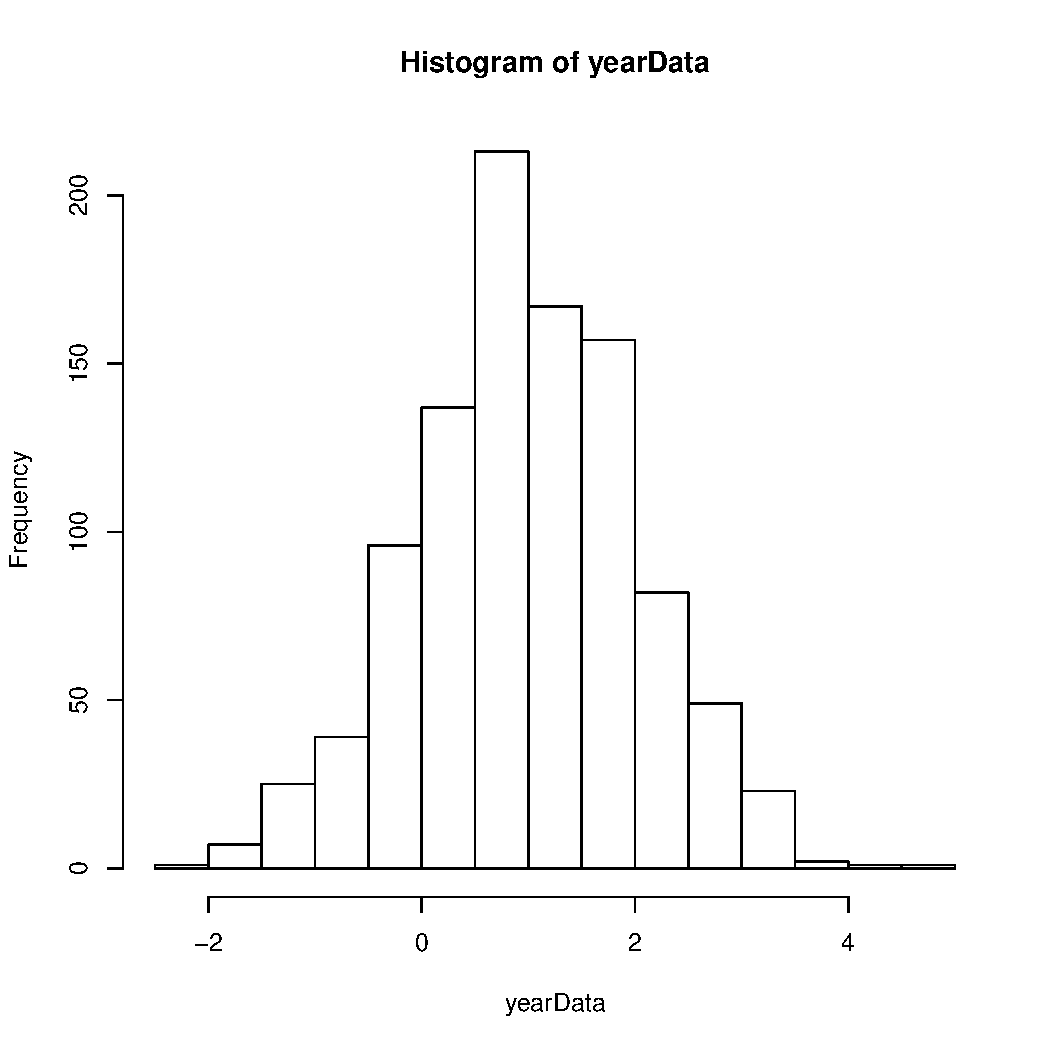
\includegraphics[width=\maxwidth]{year1/histogram-1} 

\end{knitrout}
And let's view the summary:
\begin{knitrout}
\definecolor{shadecolor}{rgb}{0.969, 0.969, 0.969}\color{fgcolor}\begin{kframe}
\begin{alltt}
\hlkwd{summary}\hlstd{(yearData)}
\end{alltt}
\begin{verbatim}
##    Min. 1st Qu.  Median    Mean 3rd Qu.    Max. 
## -2.0080  0.3026  0.9647  0.9884  1.6884  4.8103
\end{verbatim}
\end{kframe}
\end{knitrout}

